\documentclass[12pt, a4paper]{article}

% Packages
\usepackage[utf8]{inputenc}
\usepackage[bottom]{footmisc}
\usepackage[french]{babel}
\usepackage{indentfirst}
\usepackage{graphicx}
\usepackage[T1]{fontenc}


\usepackage{lscape}
\usepackage{boldline,multirow,tabularx,colortbl,diagbox,makecell,fancybox}
\usepackage{amsfonts,amssymb,amsmath,mathrsfs,array}
\usepackage{pgf,tikz,xcolor}
\usetikzlibrary{calc,positioning,shapes.geometric,shapes.symbols,shapes.misc, fit, shapes, arrows, arrows.meta,fadings,through}
%\usepackage[a4paper, top=2cm, bottom=2cm, left=2.5cm, right=2.5cm]{geometry}
\usepackage[a4paper]{geometry}
\usepackage{hyperref}
\usepackage{titlesec}
\usepackage{eurosym}
\usepackage[numbib]{tocbibind}


\tikzset{every picture/.style={execute at begin picture={
   \shorthandoff{:;!?};}
}}

\tikzset{
    boxnode/.style={ % requires library shapes.misc
        draw,
        rectangle,
        text centered,
        align=center,
        fill=gray!5!white
    },
}
\newcommand\tab[1][0.6cm]{\hspace*{#1}} %Create and define tab

\definecolor{lightgray}{gray}{0.85}
\definecolor{lightgrey}{gray}{0.85}
\definecolor{vlg}{gray}{0.85}


%Patch pour utiliser des équations dans les titres sans que hypperref nous insulte.
% Définition cyclique, compile pas. Mais c'est l"idée
%\renewcommand{\chapter}[1]{\chapter{\texorpdfstring{#1}}}
%\renewcommand{\section}[1]{\section{\texorpdfstring{#1}}}
%\renewcommand{\subsection}[1]{\subsection{\texorpdfstring{#1}}}
%\renewcommand{\subsubsection}[1]{\subsubsection{\texorpdfstring{#1}}}

%Chapter No Numbering but appears in TOC
\newcommand{\chapternn}[1]{\chapter*{#1}\addcontentsline{toc}{chapter}{#1}}
\newcommand{\sectionnn}[1]{\section*{#1}\addcontentsline{toc}{section}{#1}}
\newcommand{\subsectionnn}[1]{\subsection*{#1}\addcontentsline{toc}{subsection}{#1}}
\newcommand{\subsubsectionnn}[1]{\subsubsection*{#1}\addcontentsline{toc}{subsubsection}{#1}}

\newcolumntype{L}[1]{>{\raggedright\arraybackslash\hspace{0pt}}p{#1}}
\newcolumntype{R}[1]{>{\raggedleft\arraybackslash\hspace{0pt}}p{#1}}
\newcolumntype{C}[1]{>{\centering\arraybackslash\hspace{0pt}}p{#1}}


\renewcommand\thesection{\arabic{section}}
\renewcommand\thesubsection{\thesection.\arabic{subsection}}

%------- Do not append new commands after :

\hypersetup{	
    colorlinks=false, % colorise les liens
    linkbordercolor={1 1 1},
    breaklinks=true, % permet le retour à la ligne dans les liens trop longs
    urlcolor=blue, % couleur des hyperliens 
    linkcolor=black,	% couleur des liens internes 
    citecolor=black,	% couleur des références 
    pdftitle={}, % informations apparaissant dans 
    pdfauthor={}, % les informations du document
    pdfsubject={}	% sous Acrobat. 
}
\AtBeginDocument{\def\varmaintitle{
    \textbf{\Huge{Rapport de projet}}
}

\def\varmainsubtitle{
    \LARGE{Logiciel de clavardage en Java : conception, développement et déploiement}
}

\def\varcovertext{
    Rédigé par :
    \bigskip
    
    Enjalbert Matéo  -  Gasc Mayeul
    
    \vspace{1cm}
    
    \begin{center}
        -\hspace{0.25cm}Version du \today\hspace{0.25cm}-
    \end{center}
}
\pagenumbering{gobble}
\thispagestyle{empty}
\definecolor{insa_blue}{RGB}{52,83,111}
\definecolor{insa_red}{RGB}{226,50,46}
\noindent\begin{tikzpicture}[remember picture, overlay, shift={(current page.south west)}]
    %\draw[draw=none, fill=blue] (0,7) -- (16.7,15.75) -- (0,24.5) -- cycle;
    \draw[draw=none, path fading=east, left color=insa_blue, right color=insa_blue!10!white] (0,7) -- (16.7,15.75) -- (0,24.5) -- cycle;
    \draw[draw=none, path fading=east, left color=insa_blue, right color=insa_blue!10!white] (0,10.3) -- (14.8,18) -- (0,25.7) -- cycle;
    \draw[draw=none, path fading=east, left color=insa_blue, right color=insa_blue!25!white] (21,16.2) -- (14,19.75) -- (21,23.1) -- cycle;
    \draw[draw=none, path fading=east, left color=insa_blue, right color=insa_blue!60!white] (21,17.3) -- (7.3,24.5) -- (18.7,29.7) -- (21,29.7) -- cycle;
    \draw[draw=none, fill=insa_red] (6.5,0) -- (6.5,1.7) -- (13.5,0) -- cycle;
    \node[anchor=north west, align=right, text width=10cm] at (10,12) {\varmaintitle};
    \node[anchor=north west, align=right, text width=14cm] at (6,10.5) {\varmainsubtitle};
    \node[anchor=north west, align=center, text width=12cm] at (4.5,7) {\varcovertext};
    \node[anchor=north west] at (2,27.7) {
\includegraphics[scale=0.25]{cover/meta/logo_insat.pdf}};
\end{tikzpicture}
\newpage \pagenumbering{arabic}}

\AtEndDocument{\newpage
\pagenumbering{gobble}
\thispagestyle{empty}
\definecolor{insa_blue}{RGB}{52,83,111}
\definecolor{insa_red}{RGB}{226,50,46}
\noindent\begin{tikzpicture}[remember picture, overlay, shift={(current page.south west)}]
    \draw[draw=none, path fading=east, left color=insa_blue, right color=insa_blue!25!white] (21,7.3) -- (4.3,16.05) -- (21,24.8) -- cycle;
    \draw[draw=none, path fading=east, left color=insa_blue, right color=insa_blue!60!white] (0,16.2) -- (7,19.75) -- (0,23.1) -- cycle;
    \draw[draw=none, path fading=east, left color=insa_blue, right color=insa_blue!25!white] (0,17.3) -- (13.7,24.5) -- (2.3,29.7) -- (0,29.7) -- cycle;
    
    
    \draw[draw=none, fill=insa_red] (6.2,0) -- (6.2,1.2) -- (11.6,0) -- cycle;
    
    \node[anchor=south west, align=left] at (1.25,3.6) {\textbf{INSA Toulouse}};
    \node[anchor=south west, align=left] at (1.25,2.20) {135, Avenue de Rangueil \\ 31077 Toulouse Cedex 4 - France \\ \href{http://www.insa-toulouse.fr}{www.insa-toulouse.fr}};
    
    \node[anchor=south west] at (11.1,2.2) {
\includegraphics[height=1cm, keepaspectratio]{cover/meta/univ.png}};
    \node[anchor=south west] at (13.4,2.2) {
\includegraphics[height=1cm, keepaspectratio]{cover/meta/ministere.png}};
\end{tikzpicture}}


\begin{document}
    \begin{titlepage}
        \begin{center}
            \vspace*{1cm}
            
            \textbf{\large Rapport de projet}
            
            \vspace{0.5cm}
            
            \textbf{Logiciel de clavardage en Java : conception, développement et déploiement}
    
            \vspace{0.5cm}
    
            Matéo Enjalbert (menjalbe@insa-toulouse.fr) \\ 
            Mayeul Gasc (gasc@insa-toulouse.fr)
    
            \vfill
                
            Projet de quatrième année IR
                
            \vspace{0.8cm}
            
            
\includegraphics[width=0.4\textwidth]{logo-insa.jpg}
            
            \vspace{0.8cm}
            
            DGEI\\
            INSA Toulouse\\
            Version du \today
                
       \end{center}
    \end{titlepage}
    
    \newpage
    
    \tableofcontents
    \setcounter{page}{1}
    
    \newpage
    
    \section*{Introduction}
    \label{sec:intro}
    \addcontentsline{toc}{section}{\nameref{sec:intro}Introduction}
    
    
    \textbf{Objet de Discussion Digitale (ODD)} est un logiciel de communication partiellement décentralisé, conçu et implémenté par Matéo Enjalbert et Mayeul Gasc en tant que projet de quatrième année Informatique et Réseaux à l'INSA Toulouse. Il permet un échange de messages entre utilisateurs présent sur le même réseau et il inclut des mécanismes de gestion de l'historique des messages ainsi que de découverte des utilisateurs locaux. Implémenté en Java, il est compatible avec la majeure partie des systèmes d'exploitation modernes supportant Java 11. Il est conçu pour être déployé sur un réseau d'entreprise fermé et il peut être utilisé sans connexion internet.\\
    
    Le développement de ce logiciel s'est étalé sur deux mois (décembre 2021 et janvier 2022) et a permis d'aboutir à la validation d'une majeure partie des contraintes du cahier des charges.  La méthodologie de développement s'est basée sur une méthode Agile et a fait appel à des technologies d'automatisation du développement (en particulier pour la gestion des dépendances et le déploiement du logiciel).\\ 
    
    Ce document comprend deux manuels, un pour l'utilisateur final et le responsable du déploiement du système. Ces manuels sont suivis par une synthèse de la conception du logiciel, détaillant la méthodologie, les choix technologiques et les outils de développement utilisés.
    
    
    \newpage
    \section{Manuel utilisateur}
    Expliquant le fonctionnement de base du client, ce manuel sera utile à l'utilisateur final. L'utilisateur peut utiliser les systèmes d'exploitation GNU/Linux, MacOS ou bien Windows selon ses habitudes et son choix. En suivant les instructions suivantes, vous reconnaissez avoir pris connaissance la licence\footnote{\url{https://github.com/Enjmateo/distributed_chat_system/blob/main/license}} et l'acceptez sans réserve.
    
    \subsection{Pré-requis}
    Afin de pouvoir installer le logiciel, Java en version 11 doit être installé. Pour cela, merci de se référer au site internet de l'éditeur. Alternativement, sur les systèmes GNU/Linux, l'installation du paquet \texttt{openjdk-11-jdk} est suffisante.
    
    \begin{center}
        Obtenir Java : \url{https://www.java.com/fr/download/}
    \end{center}
    
    \subsubsection{Téléchargement et installation}
    \label{install}
    La version la plus récente du logiciel peut être directement récupérée en ligne sur la page \textit{release} du répertoire GitHub :
    
    \begin{center}
        \url{https://github.com/Enjmateo/distributed_chat_system/releases}
    \end{center}
    
    Sélectionnez la version souhaitée, cliquez sur \textbf{Assets} puis sur \textbf{release.jar}. Notez que les versions \textit{nightly} ne sont pas recommandées, car moins stables, et que les différentes versions ne sont pas compatibles en elles. En cas de doute, référez-vous à votre administrateur système pour savoir quelle version installer.
    
    Pour lancer le programme, double-cliquez sur le \textbf{release.jar}, une fenêtre doit apparaître. En cas de difficultés, vous pouvez également lancer le programme depuis la console avec la commande suivante :
    \begin{verbatim}
    java -jar release.jar
    \end{verbatim}
    \vspace{-10pt}

    \subsection{Initialisation}
    \label{config}
    Lors du premier lancement, l'utilisateur devra importer le fichier de configuration fourni par l'administrateur. Pour cela, il doit choisir \textit{Change config file} sur la première fenêtre (voir figure \ref{login1}, page \pageref{login1}).
    
    \begin{figure}[!htp]
        \centering
        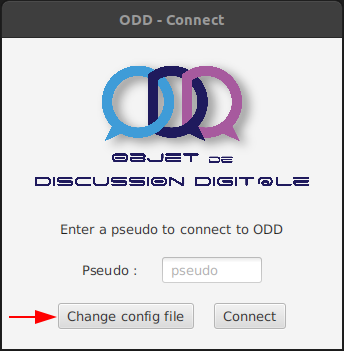
\includegraphics[width=0.47\textwidth]{img/login1.png}
        \caption{Pour mettre à jour la configuration, sélectionnez \textit{Change config file}}
        \label{login1}
    \end{figure}
    
    La configuration est alors automatiquement sauvegardée et cette manipulation n'a besoin d'être effectuée qu'une seule fois. Occasionnellement, votre administrateur réseaux peut vous demander de mettre à jour la configuration suite à la mise à jour du système. Pour la suite, merci de vous référer à la partie \textit{Utilisation} ci-après.
    
    \subsection{Utilisation}
    Dans le cas d'une utilisation courante, l'utilisateur doit commencer par choisir un pseudo. Pour cela, il renseigne dans le champ \textit{pseudo} de la première fenêtre et lance le logiciel en validant avec le bouton \textit{Connect} (voir figure \ref{login2}, page \pageref{login2}). Attention, si le pseudo déjà utilisé, l'utilisateur sera averti et devra en choisir un nouveau pseudo avant de pouvoir continuer.
    
    \begin{figure}[!htp]
        \centering
        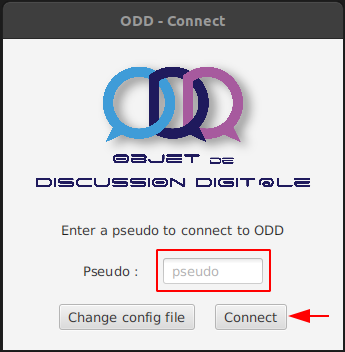
\includegraphics[width=0.47\textwidth]{img/login2.png}
        \caption{Remplissez le champ \textit{Pseudo} puis validez avec \textit{Connect}}
        \label{login2}
    \end{figure}
    
    Le client est à présent dans la fenêtre de chat principale. Sur la gauche, il voit la liste des utilisateurs connectés. Ayant sélectionné aucune conversation, la zone à droite est vide (voir figure \ref{dm}). Il peut à tous moments redimensionner la fenêtre selon ses envies en conservant une interface confortable.

    \begin{figure}[!htp]
        \centering
        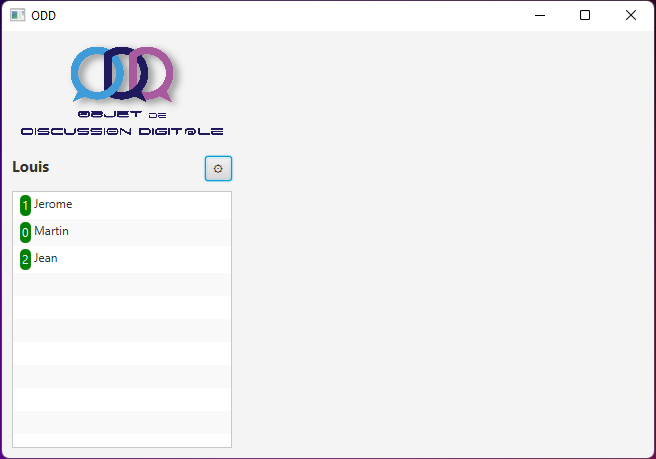
\includegraphics[width=0.85\textwidth]{img/mw/dm_window.png}
        \caption{Capture d'écran de la fenêtre principale après connexion.}
        \label{dm}
    \end{figure}
    
    Il peut converser avec n'importe quel utilisateur connecté en cliquant sur son nom. Si le client a déjà communiqué avec l'utilisateur, il voit alors l'historique de ses messages (voir figure \ref{mc}, page \pageref{mc}). Ses messages sont à droite en bleu tandis que ceux de son correspondant sont à gauche en gris. Pour envoyer un message, il suffit de le saisir dans la zone en bas puis appuyer sur la touche \textit{Enter} ou le bouton \textit{Send}.\\
    
    Le client a aussi accès au nombre de messages non lus dans les autres conversations, indiqué par un chiffre dans une bulle de couleur. Cette bulle est \textbf{verte} si l'utilisateur est connecté et \textbf{rouge} si l'utilisateur s'est déconnecté (voir figure \ref{do2}, page \pageref{do2}). Dans ce second cas, le client peut essayer de se reconnecter à l'utilisateur en lui cliquant dessus.\\
    
    \begin{figure}[!htp]
        \centering
        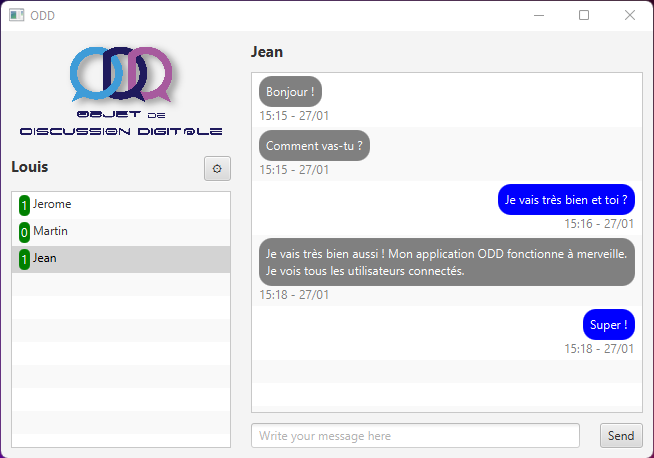
\includegraphics[width=0.85\textwidth]{img/mw/mc_window.png}
        \caption{Capture d'écran d'une conversation.}
        \label{mc}
    \end{figure}
    
    \begin{figure}[!htp]
        \centering
        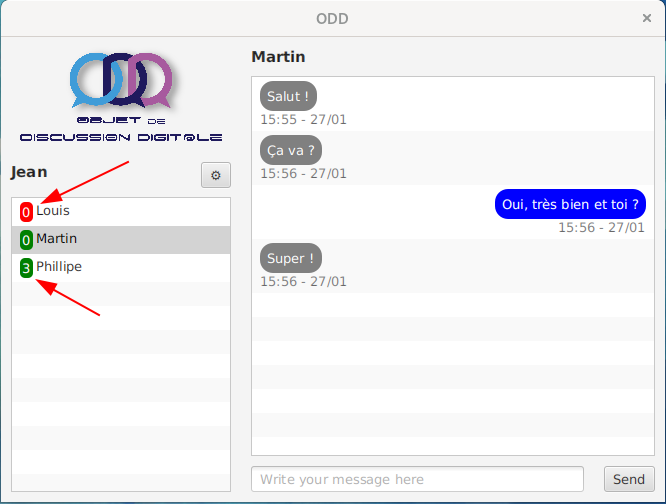
\includegraphics[width=0.85\textwidth]{img/mw/do2_window.png}
        \caption{Les flèches indiquent le statut des conversations.}
        \label{do2}
    \end{figure}
    
    \newpage
    Enfin, le client peut changer son pseudo à tout moment en cliquant sur son pseudo au-dessus de la liste des utilisateurs connectés. Il valide son nouveau pseudo avec le bouton à droite du champ \textit{Pseudo} (voir figure \ref{ps}, page \pageref{ps}).
    
    \begin{figure}[!htp]
        \centering
        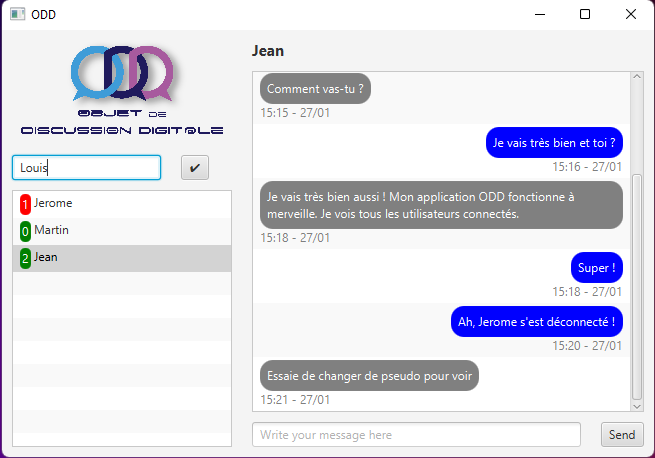
\includegraphics[width=0.85\textwidth]{img/mw/ps_window.png}
        \caption{L'utilisateur peut changer de pseudo en cliquant sur le pseudo courant.}
        \label{ps}
    \end{figure}
    
    Pour quitter le programme, il suffit à l'utilisateur de fermer la fenêtre. Les messages qu'il a envoyés seront conservés et disponibles à la prochaine ouverture du programme.
    
    
    \newpage
    \section{Manuel administrateur}
    
    \subsection{Utiliser les sources \textit{(Facultatif)}}
    Pour pouvoir apporter des modifications visuelles et/ou vous assurer de l'authenticité du programme, vous pouvez construire le programme depuis les sources. Sinon, merci de vous référer au \textit{manuel utilisateur}, section \textit{Téléchargement et installation} (page \pageref{install} de ce document).
    
    \subsubsection{Préparation}
    L'environnement de développement se base sur \textbf{Maven} pour la gestion des dépendances et \textbf{Git} pour la gestion des versions. Le module JavaFX est également utilisé pour l'interface graphique\footnote{Maven doit résoudre la dépendance. En cas de difficultés, installez JavaFX manuellement.}. Vous pouvez obtenir Maven sur le site de l'éditeur\footnote{Lien direct : \url{https://maven.apache.org/download.cgi}}. À l'instar de l'utilisateur, vous devez également disposer de Java 11.\\
    
    Sur un système Ubuntu, l'ensemble des dépendances pour être installé avec la commande suivante :
    \begin{verbatim}
    sudo apt install openjdk-11-jdk maven git
    \end{verbatim}
    \vspace{-10pt}
    
    \subsubsection{Construire depuis les sources}
    Pour construire une version spécifique, récupérez les sources sur la page \textit{release} du GitHub. Pour récupérer les dernières sources, clonez le projet sur votre machine :
    \begin{verbatim}
    git clone https://github.com/Enjmateo/distributed_chat_system
    cd distributed_chat_system/
    \end{verbatim}
    \vspace{-10pt}
    
    Vous pouvez maintenant lancer Maven :
    \begin{verbatim}
    mvn assembly:assembly
    \end{verbatim}
    \vspace{-10pt}
    
    Une fois le \textit{build} terminé, vous pouvez récupérer le JAR dans le dossier \texttt{target/}\footnote{Notez que le nom du fichier dépend de la version courante.} :
    \begin{verbatim}
    $ ls target/
    distributed_chat_system-0.0.7-jar.jar
    distributed_chat_system-0.0.7-jar-with-dependencies.jar
    \end{verbatim}
    \vspace{-10pt}
    
    Si vous souhaitez diffuser ce \textit{build}, utiliser le JAR avec dépendances.
    
    
    \subsection{Préparer l'environnement}
    \subsubsection{Base de données messages}
    Pour fonctionner avec l'ensemble des fonctionnalités (en particulier la gestion de l'historique des messages), le logiciel doit pouvoir accéder à une base de données commune. Pour configurer la base de données, l'administrateur doit utiliser le script \texttt{init\_db.sql} (disponible sur Github). Pour utiliser ce script, modifiez la première ligne par le nom de la base de données que vous souhaitez utiliser puis lancer le script :
    
    \begin{verbatim}
    mysql -u my_db_user -h my-server.com -p < init_db.sql
    \end{verbatim}
    \vspace{-10pt}
    
    Ce script permet également de réinitialiser la base de données. Ainsi, \textbf{tous les messages déjà présents seront définitivement perdus}.
    
    
    \subsubsection{Fichiers de configuration}
    Afin de simplifier la configuration pour l'utilisateur final, le logiciel accepte un fichier de configuration (voir \textit{Configuration}, page \pageref{config} de ce document). Une fois importé dans le logiciel, le fichier est conservé par le programme. Ce fichier est au format JSON et comporte trois champs :
    
    \begin{verbatim}
    {
        "dbAddr": "mysql://my-server.com/my_DB",
        "dbUser": 'my_db_user",
        "dbPassword": "my_password"
    }
    \end{verbatim}
    \vspace{-10pt}
    
    Ajustez ces champs en fonction de votre environnement et assurez-vous de mettre à disposition ce fichier de configuration aux utilisateurs.
    
    \subsubsection{Configuration réseau}
    Pour permettre la communication entre les clients, les pare-feu doivent autoriser la communication sur 3 ports au minimum :
    
    \begin{itemize}
        \item UDP 4444
        \item TCP 4445
        \item TCP 4446
    \end{itemize}
    
    \textit{\textbf{Note :} Au besoin, ces ports peuvent être modifiés dans }\texttt{utils/Consts.java}\textit{ (rebuild nécessaire). Ces ports ne sont pas filtrés par défaut sur les systèmes Debian et assimilés.}\\
    
    
    \newpage
    \section{Procédure de développement}
    \subsection{Conception}
    \subsubsection{Analyse du cahier des charges}
    Ce projet répond à un cahier des charges spécifique, la première étape de la conception a été la lecture et l'analyse de celui-ci. Il nous a donné une idée générale de ce qui était attendu, mais présentait des contraintes qui demandaient un temps de développement significativement plus élevé, nous avons donc dû faire des choix dans les spécifications implémentés. Nous avons décidé de nous en tenir à une implémentation simple (peu de sécurité, pas de portage Android, etc.) mais polyvalente et améliorable si le client souhaite investir plus de moyen sur ces points-là. De cette première étude et de ces choix, nous en avons déduit un diagramme des cas d'utilisation (voir figure \ref{ucd}, page \pageref{ucd}).\\
    
    \begin{figure}[!ht]
        \centering
        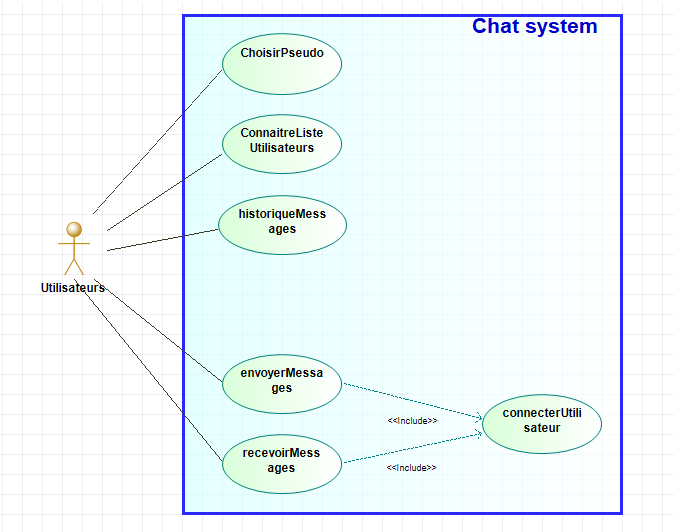
\includegraphics[width=0.8\textwidth]{img/usecases.png}
        \caption{Diagramme de cas d'utilisation réalisé sur Modelio}
        \label{ucd}
    \end{figure}
    
    \subsubsection{Structure générale}
    Durant la conception, nous avons établi des diagrammes de classe que nous avons fait évoluer tout au long de la production. Nous vous présentons ici des exemples diagrammes aboutis tels qu'ils sont en fin de production.\footnote{Nous n'avons pas pu mettre l'ensemble des diagrammes bien trop volumineux}
    
    \begin{figure}[!htp]
        \centering
        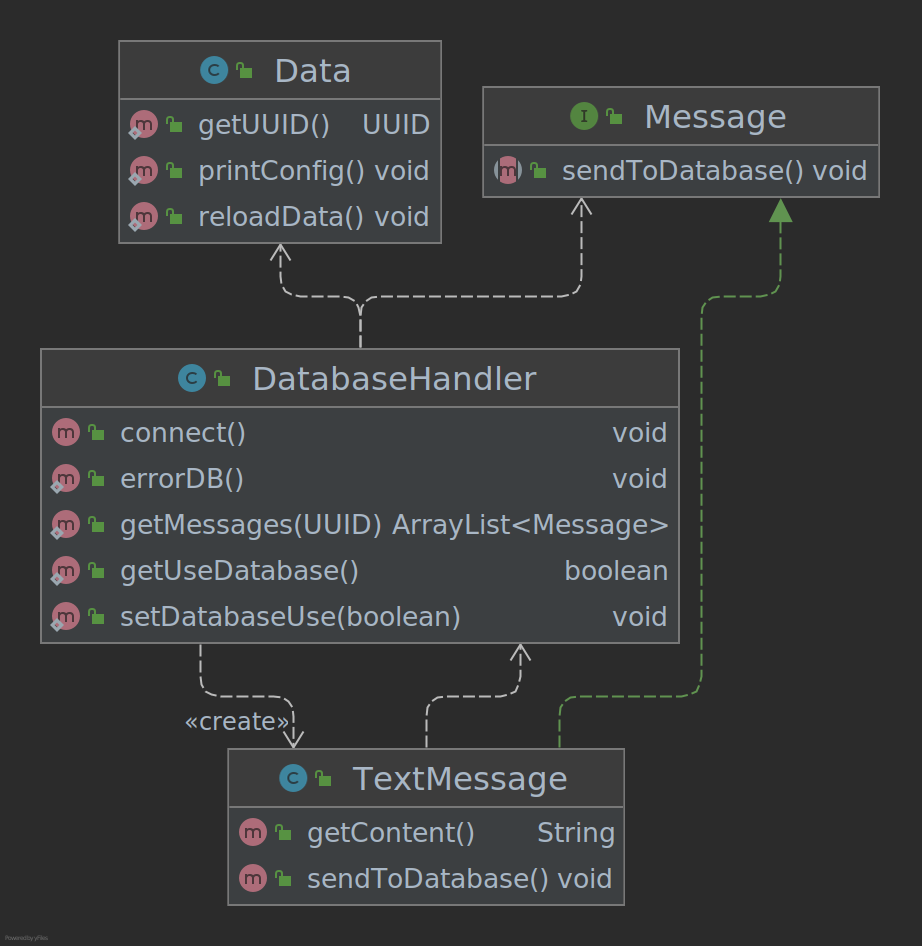
\includegraphics[width=0.48\textwidth]{img/class/communication.png}
        \caption{Diagramme de classe du package communication}
        \label{com}
    \end{figure}
    
    \begin{figure}[!htp]
        \centering
        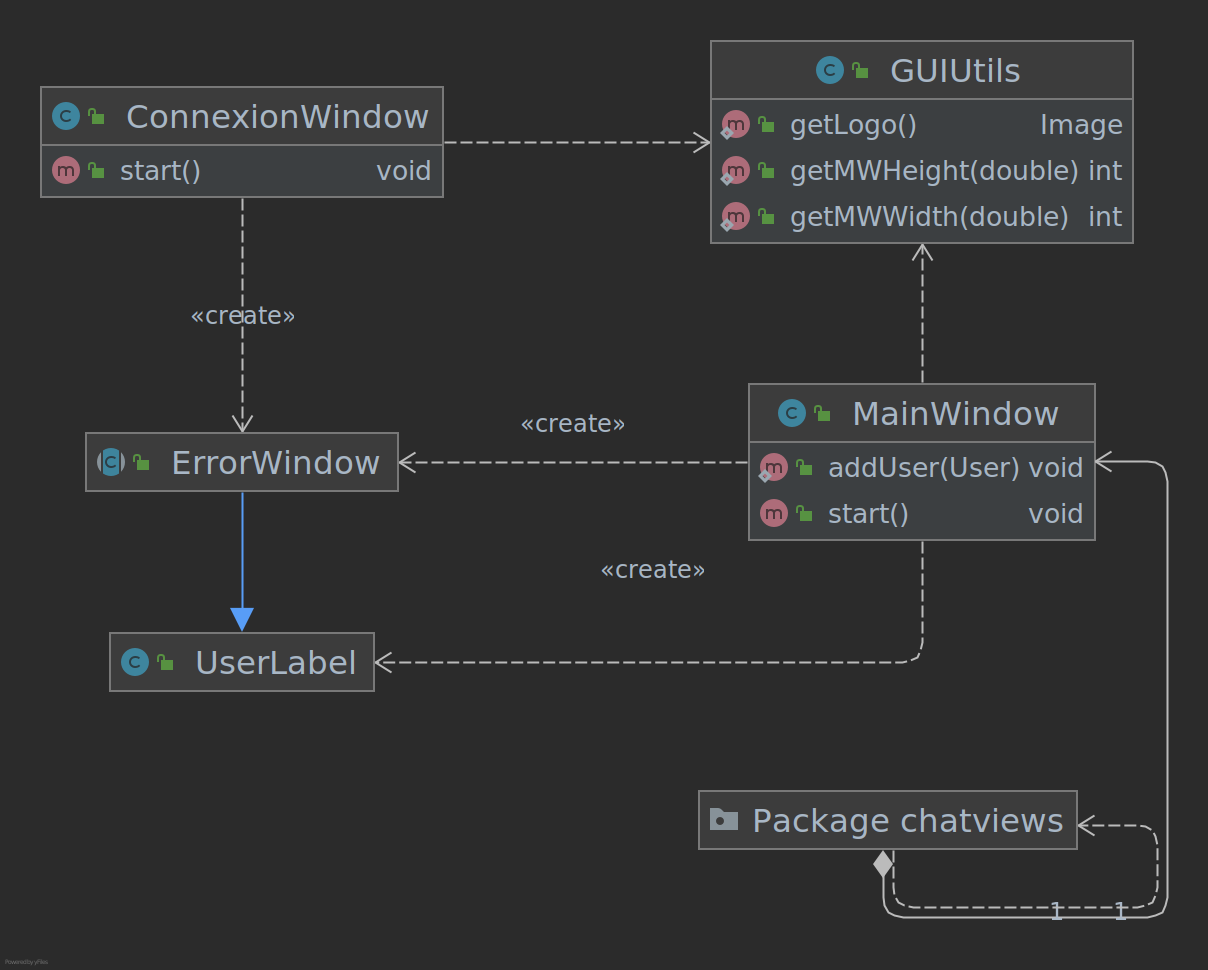
\includegraphics[width=0.58\textwidth]{img/class/gui.png}
        \caption{Diagramme de classe du package GUI}
        \label{gui}
    \end{figure}
    
    \paragraph{Package communication (voir figure \ref{com}, page \pageref{com})} Il s'agit du package responsable de la communication haut niveau, de la structure des messages et de la gestion de la base de données. Elle se repose fortement sur le package \textit{Utils} qui s'occupe pour sa part (notamment) des communications réseaux bas niveau (TCP \& UDP).
    
    \paragraph{Package GUI (voir figure \ref{gui}, page \pageref{gui})} Responsable de l'affichage de l'interface graphique à l'utilisateur, c'est la partie \textit{view} de notre modèle MVC. Deux fenêtres principales y sont définis (\textit{ConnectionWindow} et \textit{MainWindow}) et font appel à différents utilitaires, notamment \textit{GUIUtils} qui est une boîte à outil pour l'interface graphique.
    
    \subsubsection{Diagramme de séquence : découverte des utilisateurs}
    
    \begin{figure}[!htp]
        \centering
        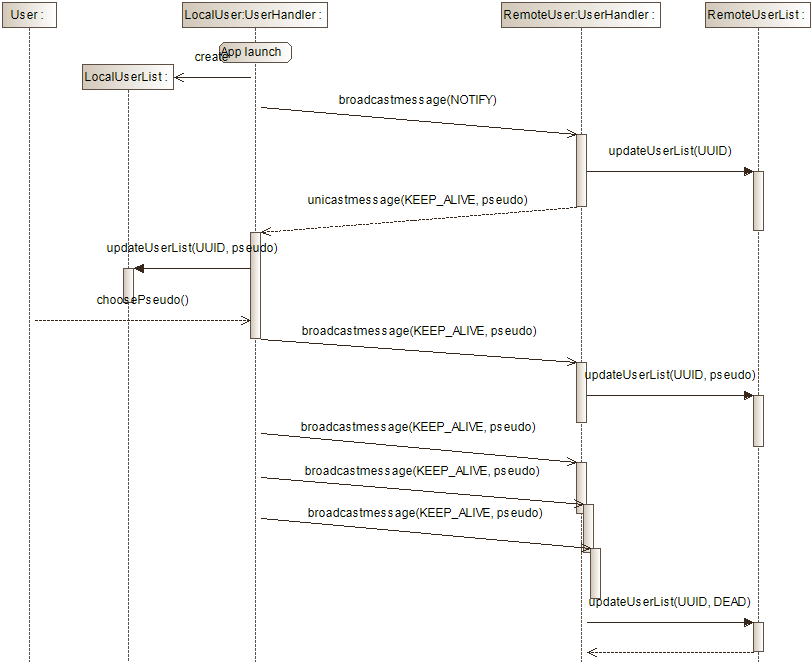
\includegraphics[width=0.97\textwidth]{img/sequence.png}
        \caption{Diagramme de séquence simplifié réalisé sous Modelio modélisant la découverte des autres utilisateurs en UDP.}
        \label{sequence}
    \end{figure}
    
    Une des particularités de notre application est son système de découverte des utilisateurs en UDP, imposé par le cahier des charges. Nous avons illustré notre implémentation par un diagramme de séquence (voir figure \ref{sequence}, page \pageref{sequence}).\\
    
    Un client qui vient de démarrer commence par broadcast un message \textit{NOTIFY} pour prévenir les utilisateurs distants de son existence. À la réception de ce message, les autres clients répondent tous un unicast \textit{KEEP\_ALIVE} au nouveau client en leur indiquant leur pseudo. À partir de ces informations, l'utilisateur peut choisir un pseudo. Une fois ce choix, le nouveau client, à l'instar des autres clients, se met à broadcast régulièrement un message \textit{KEEP\_ALIVE} avec son pseudo. Lorsque que le client s'arrête, les autres clients cessent de recevoir les \textit{KEEP\_ALIVE} et finissent par mettre à jour le client au statut \textit{DEAD}. 
    
    
    \subsection{Implémentation}
    \subsubsection{Technologies utilisées}
    Lors du développement du logiciel, nous avons été amenés à choisir entre différentes technologies. Pour effectuer ces choix, nous nous sommes basés sur nos connaissances dans le domaine et sur la qualité de la documentation à notre disposition. Nous détaillions ci-après ces différents choix.
    
    \paragraph{Maven} Nous avons retenu Maven pour la gestion du projet et la gestion des dépendances. Ce qui nous a motivé dans ce choix est la très forte capacité d'automatisation de Maven en termes de gestion des dépendances, y compris en cross-système (GNU/Linux et Windows étaient utilisés pour le développement sans problème de compatibilité).
    
    \paragraph{JDBC} Lorsque nous avions dû choisir une méthode pour gérer notre base de données, nous nous sommes tournés vers JDBC, principalement par sa simplicité d'utilisation et par sa documentation complète.
    
    \paragraph{JavaFX} Bien que nous eussions commencé le développement de l'interface graphique avec \textit{Swing}, nous avons rapidement basculé vers JavaFX, notamment pour disposer de meilleures options en termes de réactivité de l'interface, et car JavaFX offre une simplicité de développement plus intéressante.
    
    \subsubsection{Environnement de développement}
    \paragraph{IDE}
    Le projet a été développé sur \textbf{Visual Studio Code} avec l'add-on \textit{liveshare},  lequel nous a permis un processus de développement accéléré (l'add-on permettant l'édition du code en simultané avec mise à jour en temps réel). À cela venait s'ajouter \textbf{Git} pour gérer le versionnage, lequel était synchronisé avec Github\footnote{Lien Github : \url{https://github.com/Enjmateo/distributed_chat_system}}. L'avancement du projet peut donc être suivi sur la page Github du projet.
    
    \paragraph{Suivi de l'avancement}
    Le suivi de l'avancement a été effectué avec \textbf{Jira}\footnote{Lien Jira : \url{https://team-1635954518853.atlassian.net}} avec un total de 4 \textit{sprints} ayant chacun une durée comprise entre une et trois semaines. Les \textit{sprints}, établis avant le commencement du projet, étaient les suivants :
    \begin{itemize}
    \item Network 1 (Discovery \& UDP) 
    \item Network 2 (Communication \& TCP)
    \item Database (SQL)
    \item Interface utilisateur
    \end{itemize}
    Le premier \textit{sprint} est celui qui nous a pris le plus de temps, car il fallait également mettre en place l'environnement et la structure initiale. À cause de la contrainte de temps, nous avons introduit une nouvelle catégorie de ticket dans \textit{Jira} : \textit{\texttt{Reporté à plus tard}}, qui correspond aux tickets étant trop long à implémenter et que nous avons dû reporter afin de rester dans les temps.\\
    
    \textit{\textbf{Important :} Afin de permettre l'évaluation du Jira et selon instructions de l'encadrant, aucun sprint n'a été fermé. Nous avons considéré un sprint comme terminé lorsque l'ensemble des tickets étaient indiqués \texttt{Terminé} ou \texttt{Reporté à plus tard}. Notez alors que le tableau de bord n'a pas été utilisé.}
    
    \subsection{Déploiement}
    Pour des raisons de polyvalence et de facilité de déploiement, nous avons décidé d'utiliser \textbf{Github Action} en lieu et place de \textit{Jenkins} qui était recommandé pour ce projet\footnote{En faisant ce choix, nous avons consulté nos professeurs qui ont exprimé leur accord.}. Les deux systèmes ont des objectifs similaires, mais des méthodes différentes. Nos principaux usages de \textit{GitHub Action} ont été l'automatisation des \textit{builds} et le déploiement automatique des \textit{nightly} et des \textit{release} qui s'intègre directement à Github. Ainsi, notre page Github héberge les derniers \textit{builds} téléchargeables par n'importe quel utilisateur.\\
    
    La configuration de \textit{Github Action} s'effectue dans un fichier YAML (cf. \url{.github/workflows/release.yml} sur Github). Nous avons configuré trois routines, toutes déclenchées par la présence d'un tag spécifique dans le message du commit.
    
    \subsubsection{Routine \textit{Build}}
    Déclenchée par le tag \texttt{[build]} dans le message du commit, la routine prépare un environnement puis essaye de compiler le programme. La sortie de la routine informe du succès ou de l'échec de la compilation. Un exemple de sortie est fournis à la figure \ref{build_img} (page \pageref{build_img}). Au besoin, cette routine peut également être déclenchée manuellement depuis l'onglet \textit{Actions}.
    
    \begin{figure}[!ht]
        \centering
        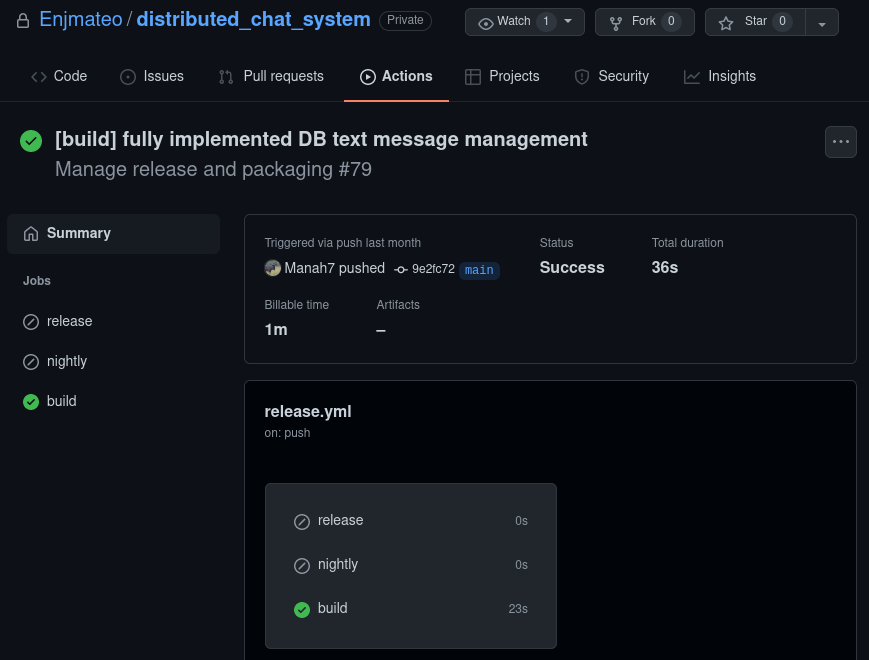
\includegraphics[width=\textwidth]{img/trigg_build.png}
        \caption{Exemple de sortie d'une routine \textit{build}}
        \label{build_img}
    \end{figure}
    
    \subsubsection{Routine \textit{Nightly}}
    Déclenchée par le tag \texttt{[nightly]} dans le message du commit, la routine effectue une compilation à l'instar de la routine \textit{Build}. Si la compilation réussie, la routine va ensuite déployer le fichier JAR produit dans une \textit{pre-release} sur Github avec la mention "nightly". Cette procédure est utile dans le cadre du développement pour déployer un fichier JAR partageable facilement. Cependant, \textbf{les fichiers produits par ces routines n'ont pas pour objectif d'être déployés en production} et sont réservés pour le développement.
    
    \subsubsection{Routine \textit{Release}}
    Déclenchée par le tag \texttt{[release]} dans le message du commit, la routine effectue un travail très similaire à la routine \textit{nightly}. La routine aboutie cependant à la publication d'une version stable sur la page \textit{Release} du Github. Ces versions sont destinées à être utilisées par le client, elle n'est cependant pas immune aux bugs et seule la \textit{release} la plus récente est recommandée.
    
    
    \subsection{Tests}
    Pour nous assurer du bon fonctionnement de notre programme avant la publication de \textit{releases}, nous avons effectué une série de tests. Nous décrivons notre méthode dans cette section.
    
    \subsubsection{Environnement de test}
    \paragraph{Tests sur les ordinateurs de développement}
    La majorité des tests, en particulier ceux effectués pendant le développement, ont été réalisés dans un environnement simulé de réseau d'entreprise. Pour cela, nous avons utilisé le logiciel \textbf{\textit{ZeroTier}} qui permet d'émuler un réseau local à travers internet.
    
    \paragraph{Tests en salle de TP}
    Nous avons également testé notre logiciel sur les machines de TP INSA, car le réseau sur lequel elles se trouvent est typé d'un réseau d'entreprise et nous a permis de valider nos tests en conditions réelles. Cependant, l'environnement de développement n'étant pas disponible sur ces machines et ne souhaitant pas mélanger les configurations IDE, nous avons privilégié l'utilisation de \textit{pre-release nightly} rapidement et simplement déployable sur ces machines. Cette configuration nous permettait également de testé la viabilité de notre package JAR.
    
    
    \subsubsection{Conclusion des tests}
    Dans les deux environnements, les tests se sont montrés concluants et les spécifications visées ont été atteintes. Nous avons notamment utilisé ODD afin d'échanger pendant la rédaction de ce rapport. Cependant, nous avons constaté que sur un réseau particulièrement instable, la connexion à la base de données présente des erreurs. Pour palier ce problème, nous avons ajouté une option au démarrage permettant d'utiliser l'application sans l'historique des messages. Dans ce cas, le fichier de configuration n'est pas requis. Cette option nous a également facilité les tests sans imposer une connexion systématique à la base de donnée. 
    
\end{document}

